% (1) Overall Correspondence of challenge 1, novelty 1, solution 1, ...
% (2) Q1: Think from demand: what are the attractive/necessary demands from the research community that have not been fully satisfied?
% (3) Q2: Relate to the community consensus/trend to show your importance. We point out the gap/potential/opportunities between the current consensus.
% (4) Q3: Crucial if you care about the impact and citations of your paper. Show your insights, help future researchers join our endeavor later. They will become your followers -- of your paper and yourself. These challenges are fundamental and have been tackled by your paper, but cannot be fully solved.
% (5) Q4: Prove your novelty: no one has solved XYZ, but we did. These limitations can be perfectly solved after your paper.
% (6) Q5: Solution XYZ to (partly) solve challenges and fill novelty gaps.

LLMs are increasingly capable of interacting with external environments, leveraging tools, and reasoning over memory, which enabled a new paradigm: LLMs Agents \citep{schick2023toolformer, qin2023toolllm, packer2023memgpt, shinn2023reflexion,liu2025advanceschallengesfoundationagents}. General purposed LLMs agents have driven advances across diverse domains, including embodied control, scientific discovery, open-ended web interaction, and research support \citep{zhou2023webarena, li2025metal, hong2025embodiedwebagentsbridging, zhu2025safescientistriskawarescientificdiscoveries}. Despite these achievements, current agents remain imperfect and insufficiently robust. They frequently exhibit errors—ranging from misinterpreting instructions and misusing tools to breaking down in long-horizon reasoning. These shortcomings underscore that, while promising, existing LLM Agents still lack the reliability required for real-world deployment. This observation motivates us to ask: \textit{\textbf{Where do LLM agents fail}} ?

While prior works have investigated the failures of LLM-based agents \citep{ji2024testing, sung2025verila, ning2024defining, cemri2025why, zhang2025which}, they have largely focused on enumerating error types or providing qualitative case studies. However, these analyses stop short of offering systematic mechanisms to trace failures back to their \textit{root causes}, and importantly, do not enable agents to fix these discovered failures based on such insights. To close this gap, we modularize error analysis with the explicit goal of tracing failures to their underlying causes. We conduct a large-scale study over hundreds of trajectories, decomposing each rollout into four operational modules: memory, reflection, planning, and action. By attributing each failure to its root module, we derive the \AET{} — a comprehensive taxonomy of failure modes designed to ground systematic error detection and guide the development of robust mitigation strategies. 

% Our highlights: modularize analysis that traces the root cause; 
% paradigm shift from offline error analysis to online error fix, crucial due to the dynamics and interactive environment: we move from purely offline error analysis, to an interface that allows debug agent to interact and fix the error only. 

\begin{figure}[htbp]
    \centering
    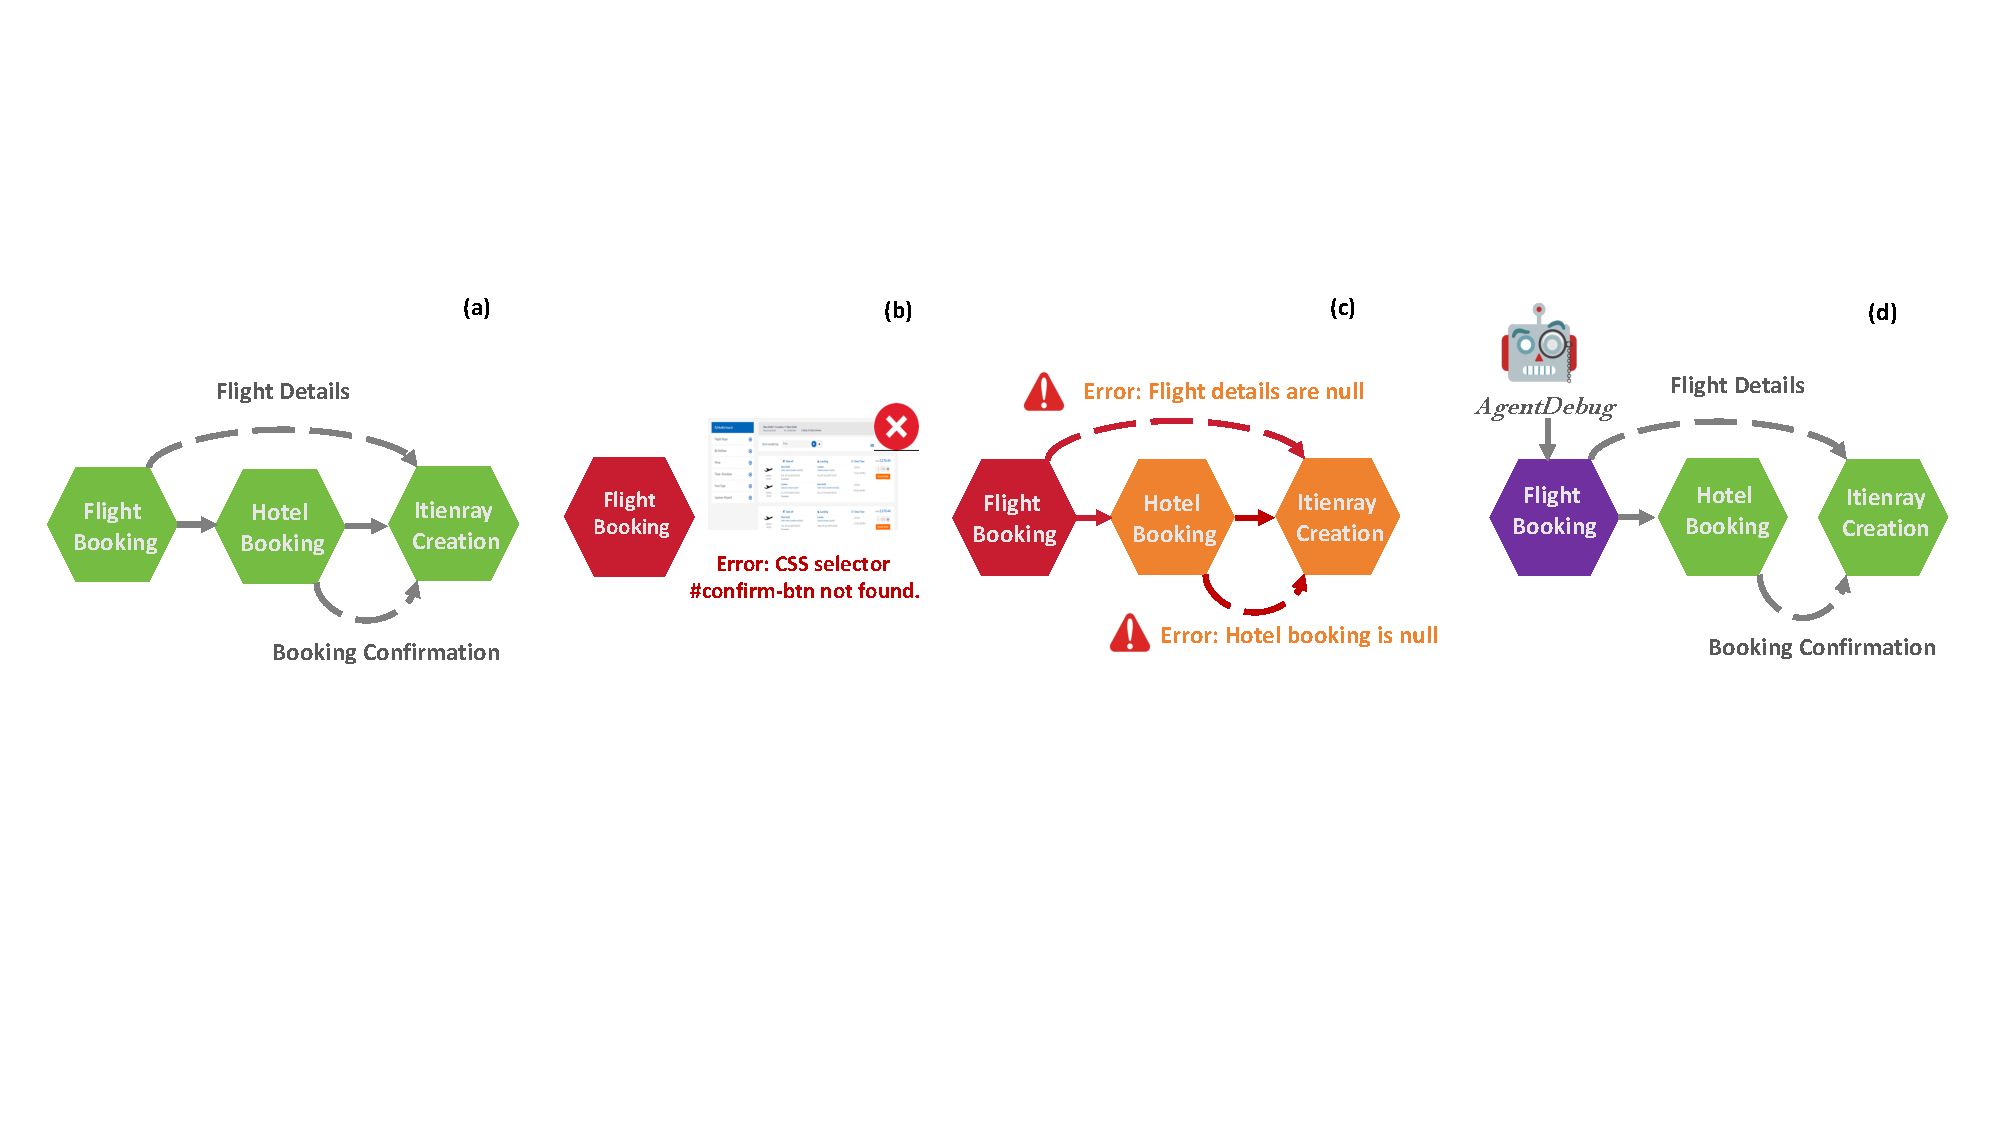
\includegraphics[width=1\linewidth]{figures/teaser.pdf}
    \caption{\textbf{\textit{Motivation for \ModelName{}}}: A single root-cause failure (b) can propagate through subsequent steps (c), compounding errors and leading to task failure. \ModelName{} (d) addresses this bottleneck by tracing failures back to their source and providing actionable feedback that enables agents to evolve into more robust versions.}
    \label{fig:teaser}
    \vspace{-0.2in}
\end{figure}


%%% We identified the key bottleneck- Error Propagation
Our analysis reveals a critical bottleneck in LLM agents: \emph{error propagation}. As illustrated in Figure~\ref{fig:teaser}, a single root-cause failure (b) can cascade into successive errors (c), compounding degradation and leading to task failure. This challenge is especially acute in long-horizon tasks, where early mistakes distort later reasoning and actions, making recovery difficult. These insights motivate our central question: \textit{\textbf{How can LLM agents refine from failures}}?

%%% Prior works 
Recent progress in LLMs agent enhancement has largely centered on expanding the reasoning search space—through chain-of-thought~\citep{wei2023chainofthoughtpromptingelicitsreasoning}, tree-of-thought~\citep{yao2023treeofthoughts}, and graph-of-thought~\citep{besta2023graphofthoughts} approaches—or on incorporating step-level self-reflection \citep{yao2022react, yao2023treeofthoughts, besta2023graphofthoughts}, which allows agents to deliberate more thoroughly and locally revise their actions. While these advances improve flexibility and reasoning depth, they typically treat the trajectory as a sequence of isolated steps rather than as a coherent, interdependent process. 

% In reality, an agent’s trajectory is more akin to a program: it unfolds step by step, with dependencies, state changes, and side effects that accumulate over time. Viewing agents in this way suggests that improving their reliability is not only a modeling challenge but also an engineering one. Just as complex software systems require systematic debugging to trace and correct root-cause errors, agent systems demand principled debugging methodologies to enhance robustness. This perspective motivates us to propose debugging as the foundational mechanism for building more reliable LLM agents.


% summarize
% One of our key observations is that in reality, an agent’s trajectory is more akin to a program: it unfolds step by step, with dependencies, state changes, and side effects that accumulate over time. Viewing agents in this way suggests that improving their reliability is not only a modeling challenge but also an engineering one. Just as complex software systems require systematic debugging to trace and correct root-cause errors, agent systems demand principled debugging methodologies to enhance robustness. This perspective motivates us to propose debugging as the foundational mechanism for building more reliable LLM agents.

To address this challenge, we propose \ModelName{}, a debugging framework that decomposes a trajectory into decision steps, isolates the minimal set of root-cause failures, and provides corrective feedback back to the responsible states or actions. This process not only reduces noise from irrelevant errors but also highlights the key weaknesses that hinder successful task completion. As illustrated in Figure~\ref{fig:teaser} (d), \ModelName{} enables agents to iteratively evolve into more robust versions by learning directly from their failure cases. To rigorously evaluate whether models can detect critical errors and produce actionable feedback, we also construct the \Bench{}. This benchmark grounds the taxonomy in real-world trajectories, offering the first standardized testbed for error detection and debugging.

%%% Experiment summary
We evaluate \ModelName{} on \Bench{}, where it achieves 24\% higher all-correct accuracy (24.3\% vs. 0.3\%) and 17\% higher step accuracy (45.0\% vs. 28.0\%) compared to the strongest baseline. Beyond detection, the targeted feedback generated by \ModelName{} enables agents to iteratively recover from failures, yielding up to 26\% relative improvements in task success across ALFWorld, GAIA, and WebShop. Ablation studies further confirm that focusing on root-cause errors, rather than attempting to fix every surface-level mistake, is key to efficient debugging and meaningful performance gains.
%%%% Contribution
Overall, our contributions are summarized as follows:
\begin{itemize}[leftmargin=1.2em, itemsep=0.1em, topsep=0.25em]
    \item We analyze failed trajectories of LLM agents across diverse benchmarks and show that error propagation—early mistakes cascading into later failures—is the key bottleneck to robustness. From this study, we derive the \AET{}, a unified taxonomy of failure modes spanning planning, tool use, memory, and reflection.
    \item We introduce \Bench{}, the first curated dataset of systematically annotated failures from ALFWorld, GAIA, and WebShop. Each trajectory is labeled with fine-grained error categories and actionable feedback, providing a standardized testbed for studying, benchmarking, and comparing agent debugging methods.
    \item We present \ModelName{}, a debugging framework that identifies critical errors and provides actionable feedback. \ModelName{} achieves high root-cause detection accuracy, exceeding strong baselines by 24\%, and improves task success rates by 26\% across embodied reasoning, web interaction, and decision-making domains.
\end{itemize}
